\begin{landscape}
\begin{figure}
\centering
  \begin{tikzpicture}[node distance=2mm,scale=1, every node/.style={scale=1}]
  \begin{scope}[start chain]
    \node[minimum height=10cm,   minimum width=4.4cm,  on chain, text width=4cm, draw, name=KP]  (0,0)                  
    {\scriptsize \textbf{Key Partners:}\\ 
We want partners like Valk Welding who are suppliers of robot welding systems with a broad network. For hardware, no specific supplier is intended.
    }; 
      \begin{scope}[start branch]
	\node[minimum height=4cm,   minimum width=11.3cm,    on chain=going below, text width=9.5cm, draw, name=CoS,xshift=3.45cm] 
	{\scriptsize\textbf{Cost Structure:}
There are fixed costs in rental of premises, employees and etc. A big part of the cost structure is variable, it varies with the revenue. Like procurement of supplies which is coherent with sales. 
	}; 
	\node[minimum height=4cm,   minimum width=11.34cm,    on chain=going right, text width=9.5cm, draw, name=RS]  
	{\scriptsize\textbf{Revenue Streams:}\\
A revenue stream is generated through the sales channel to the various robot-developing companies, who end up providing the product to the end customers.
We will develop our product for specific welding robots for a price, providing another potential revenue stream. 
Patenting the product will be also an important part to maintain revenue, as it will allow us to charge a significant sum of money from companies who wish to use our technology.
	}; 
      \end{scope}
      
      
      \begin{scope}[start branch]
	\node[minimum height=4.84cm, minimum width=4.4cm,  on chain=going right, text width=4cm, draw, name=KA,yshift=2.58cm]     
	{\scriptsize\textbf{Key Activities:}\\
Initially, the main activity will be development of concept, later on the focus will shift to manufacturing of the product in parallel with improvement of concept for optimal market/customer fitness.
	};
      \end{scope}
      \node[minimum height=4.84cm, minimum width=4.4cm,  on chain=going right, text width=4cm, draw, name=KR,yshift=-2.58cm]              
      {\scriptsize\textbf{Key Resources:}
In the development phase we need start-up capital. Reliable suppliers is a must in order to have a reliable business. A robot welding company as partner is preferred. 
      }; 
      \node[minimum height=10cm,   minimum width=4.4cm,  on chain=going right, text width=4cm, draw, name=VP,yshift=2.58cm]                
      {\scriptsize\textbf{Value Proposition:}
We offer a flexible way to program welding robots. Which provides quality welding, efficiency, easy setup and training, reduction in quality controls and a significant reduction in labour hours.
      };
	\begin{scope}[start branch]
	  \node[minimum height=4.84cm, minimum width=4.4cm,  on chain=going right, text width=4cm, draw, name=CR,yshift=2.58cm]              
	  {\scriptsize\textbf{Customer Relationship:}
We will have contact to our customers through feedback from end users. This will help us improve/maintain market fitness.
	  }; 
	\end{scope}
      \node[minimum height=4.84cm, minimum width=4.4cm,  on chain=going right, text width=4cm, draw, name=Ch ,yshift=-2.58cm]              
      {\scriptsize\textbf{Channels:}\\
End users buy our product through welding robot companies/sellers. We will be participating in relevant conferences with partners. Provide a website with technical information of product, videos, contact information and etc.. Contact can also be by phone, email, chat/online support.	
      };
      \node[minimum height=10cm,   minimum width=4.4cm,  on chain=going right, text width=4cm, draw, name=CuS,yshift=2.58cm]               
      {\scriptsize\textbf{Customer Segments:}\\
Relevant customers are companies who are already in the zone of robotic welding, companies who could be interested in buying the product to supplement their own products. Primarily it will be customers who develop either robots or other technical parts for them.  
Our end users will be SME's who uses welding with a frequent replacement of production.
      };
    \end{scope}
    

  \end{tikzpicture}
  \caption{Osterwalder Business Model}
  \label{ost_business_model}
\end{figure}
\end{landscape}

% \subsubsection{Customer segment}
% Relevant customers are companies who are already in the zone of robotic welding, companies who could be interested in buying the product to supplement their own products. Primarily it will be customers who develop either robots or other technical parts for them.  
% Our end users will be SME's who uses welding with a frequent replacement of production.
% \subsubsection{Value proposition}
% We offer a flexible way to program welding robots. Which provides quality welding, efficiency, easy setup and training, reduction in quality controls and gives a significant reduction in labour hours.
% \subsubsection{Channels}
% End users buy our product through welding robot companies/sellers. We will be participating in relevant conferences with partners. Provide a website with technical information of product, videos, contact information and etc.. Contact can also be by phone, email, chat/online support.	
% \subsubsection{Customer relationships}
% We will have contact to our customers through feedback from end users. This will help us improve/maintain market fitness.
% \subsubsection{Revenue}
% A revenue stream is generated through the sales channel to the various robot-developing companies, who end up providing the product to the end customers.
% We will develop our product for specific welding robots for a price, providing another potential revenue stream. 
% Patenting the product will be also an important part to maintain revenue, as it will allow us to charge a significant sum of money from companies who wish to use our technology.
% \subsubsection{Key resources}
% In the development phase we need start-up capital. Reliable suppliers is a must to have a reliable business. A robot welding company as partner is preferred. 
% \subsubsection{Key activities}
% Main activity in the beginning will be development of concept, later on it will be production of concept in parallel with improvement of concept for optimal market/customer fitness.
% \subsubsection{Key partners}
% We want partners like Valk Welding who is a robot welding company with a broad network. For supplies, no specific supplier is intended.
% \subsubsection{Costs}
% Where are fixed costs in rental of premises, employees and etc. A big part of the cost structure is variable, its varies with the revenue. Like purchasing of supplies which is coherent with sales. 
\subsection{Business Model}
The business model (based on the Osterwalder business model) is providing a short overview of the business plan. It will help to the company to create, deliver and capture value in economic and other contexts. It is also useful to represent core aspects of a business, such us, purpose, target customers, strategies, etc.  The model is divided into 9 categories: 
\begin{table}[h!]
\begin{tabular}{c c}
\begin{minipage}{8cm}
\begin{enumerate}
\item Key Partners
\item Key Resources
\item Key Activities
\item Value Proposition
\item Channels
\end{enumerate}
\end{minipage}
&
\begin{minipage}{8cm}
\begin{enumerate}[]
\item [6.] Customer Segments
\item [7.] Customer Relationships
\item [8.] Cost Structure
\item [9.] Revenue Stream
\end{enumerate}
\end{minipage}
\\
\end{tabular}
\end{table}

\subsection{Idea and Background}
This section briefly covers a description of the problem that we are trying to solve, how we are going to solve it.

It will also contain a short presentation of members of the team and an explanation as to why we are the perfect fit for this start up company.

\subsubsection{The Team}
We are a dedicated team of engineering students. We believe that we have the drive and expertise necessary to realise this project. This project is an extension of our individual interests and as such it is only natural that we extend this to our proffesional careers. Below is a presentation of all of the members of the team.

\begin{table}[h]
\centering
\begin{tabular}{|c|c|c|c|}
\hline
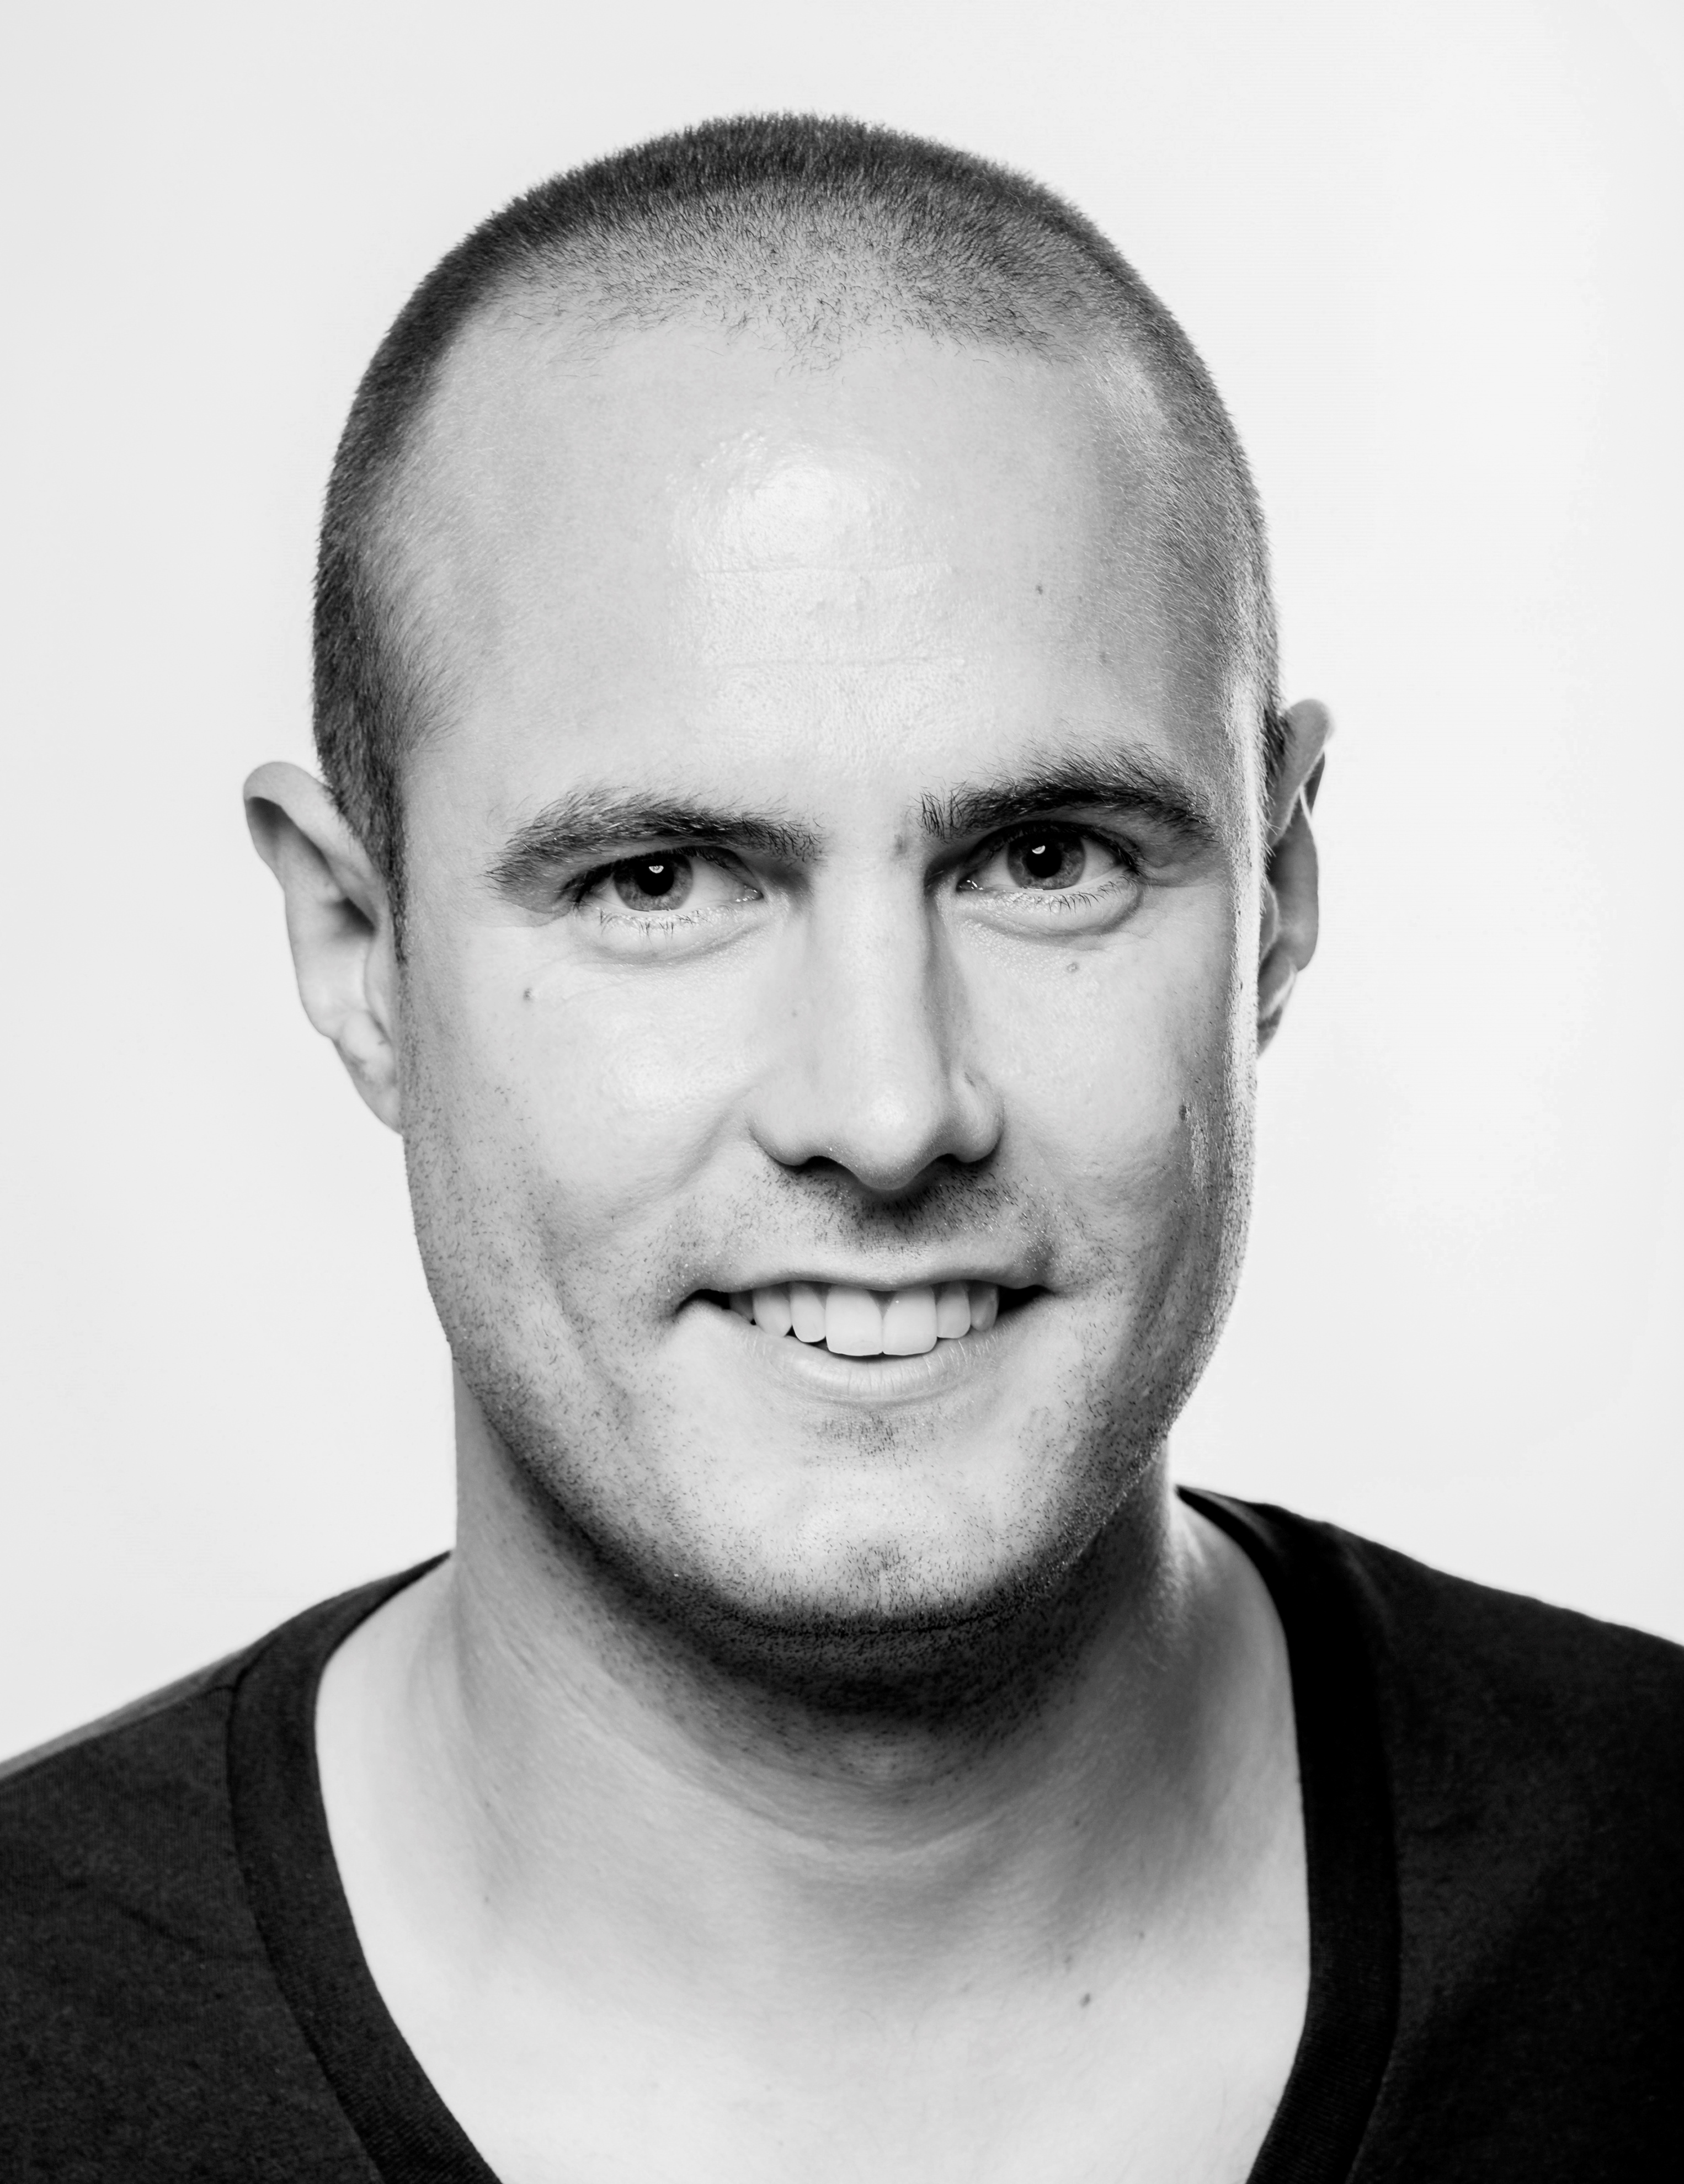
\includegraphics[width=0.2\textwidth]{graphics/cgopic} & %casper

\includegraphics[width=0.2\textwidth]{graphics/AnonProfile} & %david
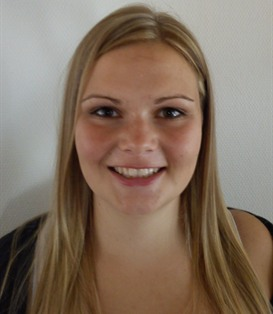
\includegraphics[width=0.2\textwidth]{graphics/Kirstine} & %kirstine
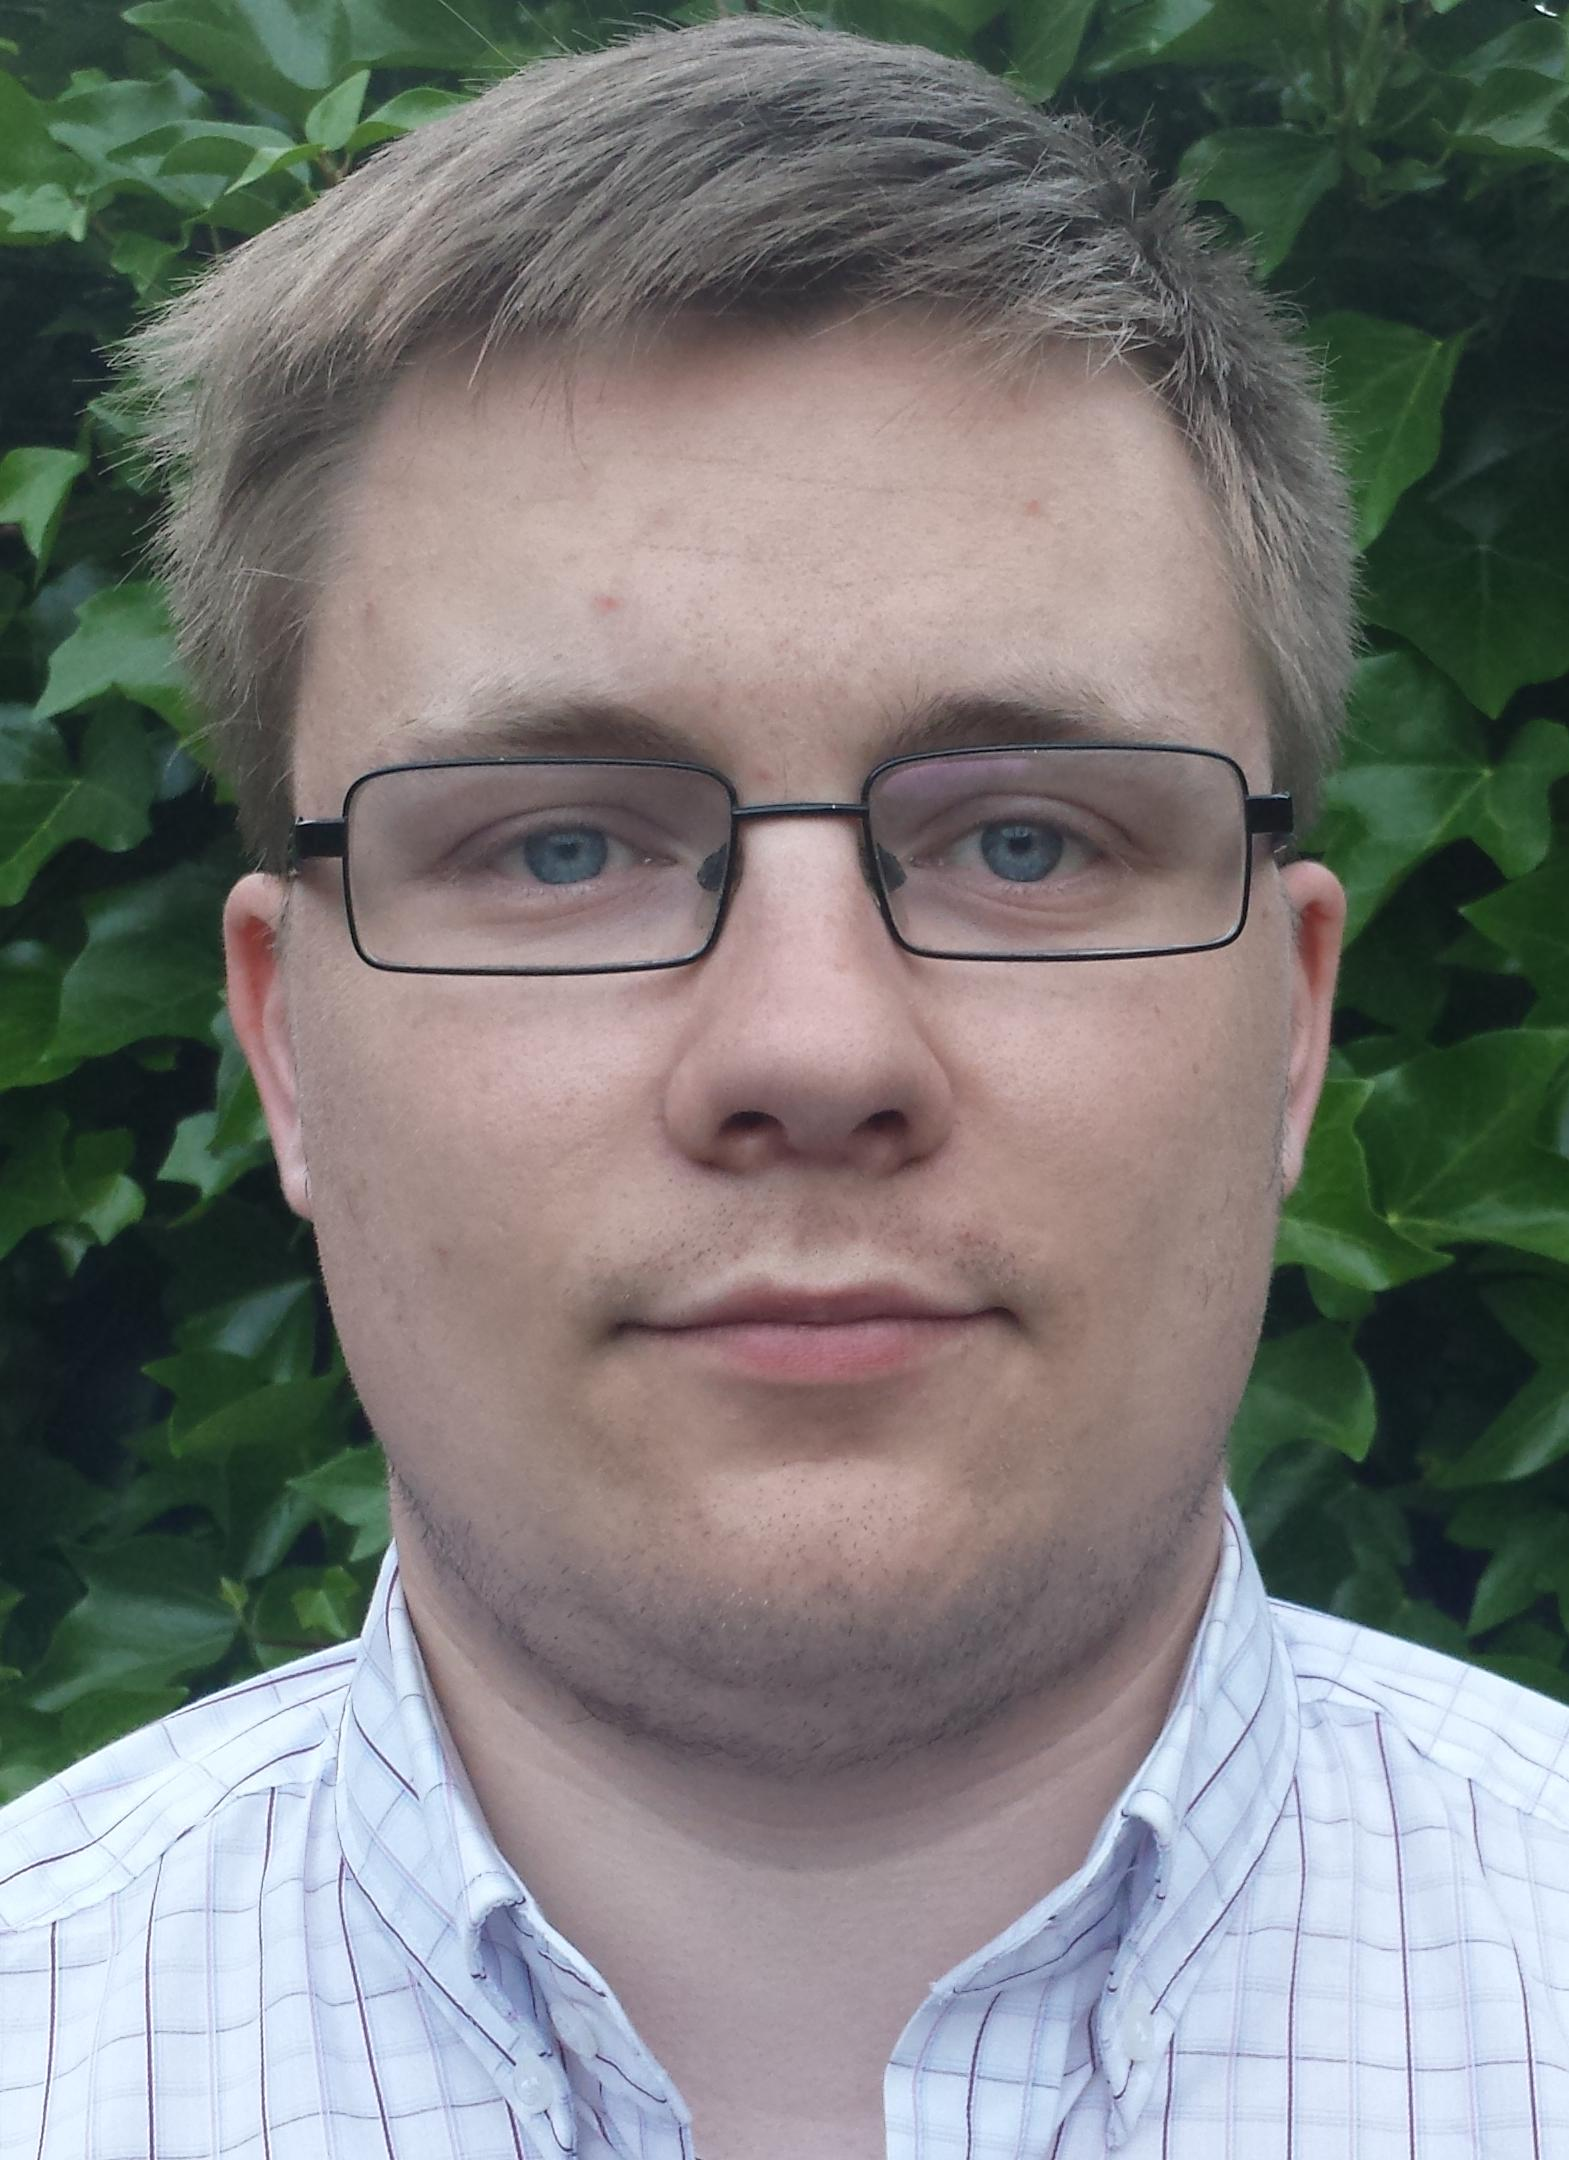
\includegraphics[width=0.2\textwidth]{graphics/Nikolaj_profile} \\ \hline %nikolaj
\parbox[t] {0.2\textwidth}{
\textbf{Casper:} \\
28 years old, originally from Gelsted, Denmark. Educated Electrician. Studying Energy Technology.
}

&

\parbox[t] {0.2\textwidth}{
\textbf{David:} \\

} 

&

\parbox[t] {0.2\textwidth}{
\textbf{Kirstine:} \\
I am 22 years old. Originally from Kolding, Denmark. I study M.Eng in Physics and Technology.
} 

&

\parbox[t] {0.2\textwidth}{
\textbf{Nikolaj:} \\
I am 24 years old and originally from Esbjerg, Denmark. I am currently studying M.Eng in Robotic Systems.
} 

\\\hline
\end{tabular}

\begin{tabular}{|c|c|c|}
\hline
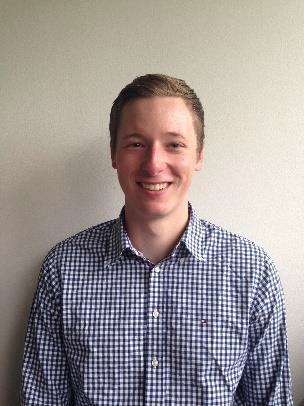
\includegraphics[width=0.2\textwidth]{graphics/Simon_profile} & %simon

\includegraphics[width=0.2\textwidth]{graphics/AnonProfile} & %thomas
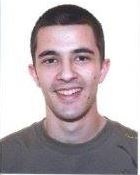
\includegraphics[width=0.2\textwidth]{graphics/sexy_xabi_profile} \\ \hline %xabier
\parbox[t] {0.2\textwidth}{
\textbf{Simon:} \\
I am 23 years old and originally from Haderslev, Denmark. Currently studying IT-Engineering.

} 

&

\parbox[t] {0.2\textwidth}{
\textbf{Thomas:} \\
Age: 26, from Tønder. I'm currently studying to become M.Eng in Robotic Systems
} 

&

\parbox[t] {0.2\textwidth}{
\textbf{Xabier:} \\
I am 21 years old and originally from Bilbao, Spain. I am currently studying Industrial Engineering.
} 

\\\hline
\end{tabular}
\end{table}



\subsubsection{Passion}
With a team profile that covers most roles, the group is well balanced. One of our main strengths is the analytical skills and assets of our specialists, which form more than half of the team.  
With skills such as programming, knowledge within the field of robots, software designing and lasers, each development challenge is within our area of expertise. 
Our motivation is the very real possibility that we will create a product that will provide the industry, not only with a highly flexible welding solution, but also the basis for an entirely new application of existing technologies that could be employed in many other industries.
It is our conviction that we are the right team to bring together this range of technologies to create something new, exiting and potentially highly lucrative.